%\documentclass{article}
\documentclass[11pt, letterpaper, twoside]{article}
\usepackage[utf8]{inputenc}
\usepackage{graphicx}
\usepackage{subcaption}
\usepackage{booktabs}
\usepackage[margin=1in]{geometry}
\usepackage[justification=centering]{caption}
\usepackage{cprotect}
\usepackage{amsmath}

% Page 1
\title{CTA200H Computing Project}
\author{Eegene Chung}
\date{May 21, 2019}

\begin{document}
\maketitle

% Question 1
\section{Exploring Theoretical Matter Power Spectra}

The effects of different cosmology parameters - redshift $z$ (\verb|z|), baryonic matter density $\Omega_m h^2$ (\verb|ombh2|), cold dark matter density $\Omega_c h^2$ (\verb|omch2|), and total neutrino mass $M_\nu$ (\verb|mnu|) - on the matter power spectra $P_m(k)$ will be shown using the \verb|camb| package for Python.\\\\

We first want to know what representation of the power spectra will be the most informative. To show this, the matter power spectrum at redshift $z = 0$, $H_0 = 67.5$, $\Omega_m h^2 = 0.022$, $\Omega_c h^2 = 0.122$ is plotted first using a linear $x, y$ scale, then a logarithmic scale.

% Figure 1
\begin{figure}[h!]
    \centering
    % Subfigure (a)
    \begin{subfigure}[b]{0.47\textwidth}
        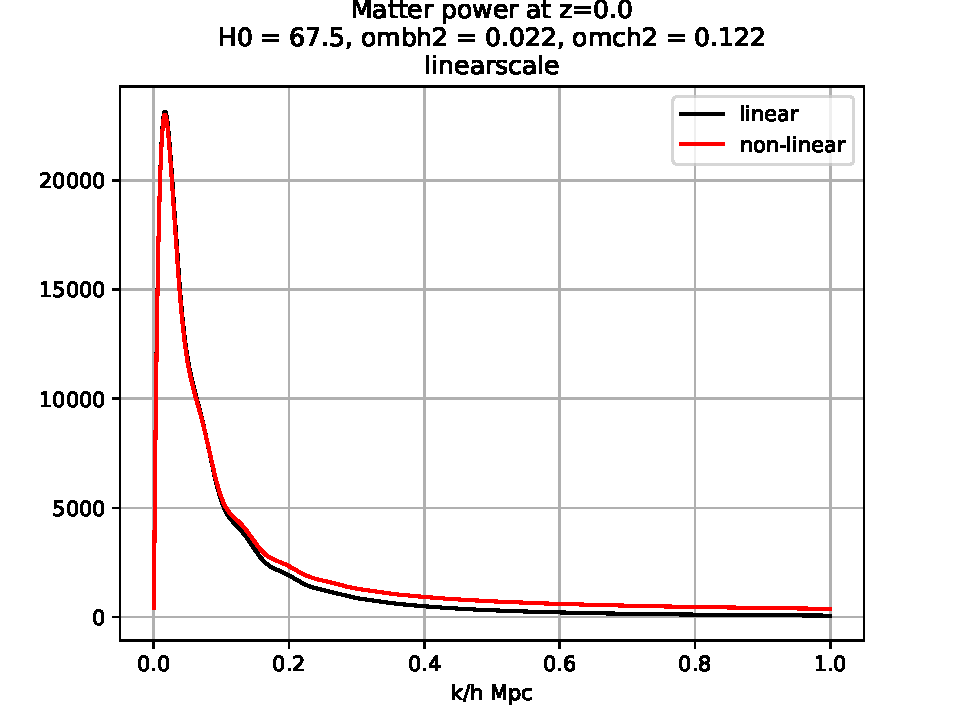
\includegraphics[width=\linewidth]{powerspectrum_linearscale.pdf}
        \caption{Linear Scaling}
    \end{subfigure}
    % Subfigure (b)
    \begin{subfigure}[b]{0.47\textwidth}
        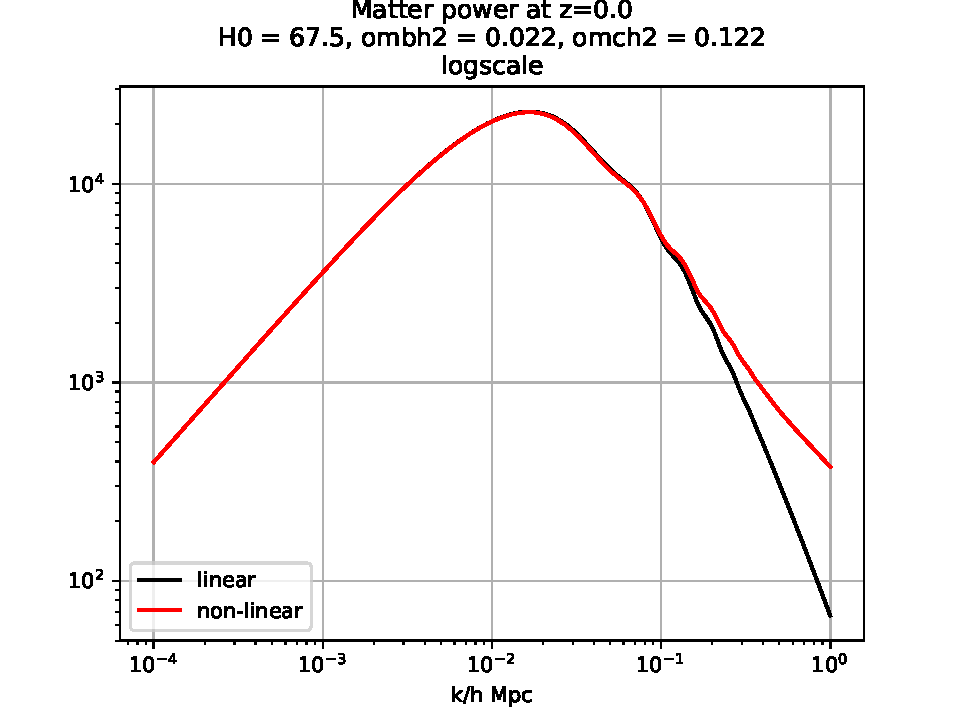
\includegraphics[width=\linewidth]{powerspectrum_logscale.pdf}
        \caption{Logarithmic Scaling}
    \end{subfigure}
    \caption{Matter power spectrum plotted with different scaling\\ showing the effect of linear and nonlinear growth}
    \label{fig:log_lin_scale}
\end{figure}

Figure 1 (a) shows the matter power spectra using a linear scaling for both axes. Here, it is hard to notice the slight oscillatory motion near the peak because the curve is so steep. As well, although it can be seen that the linear and non-linear deviate from each other for $k$ above approximately $0.1$, it does not seem very significant. In Figure 1 (b), the same power spectra was graphed using a logarithmic scale for both axes. This plot shows a clear divide in the spectra for $k$ above $10^-1$, as well as the distinctive oscillatory motion for $k$ above $10^-2$. Therefore, it is much more useful to use logarithmic scaling to plot the power spectra.\\\\
\newpage

% Page 2
Now, we will explore the impact on the theoretical power spectra $P_m(k)$ by changing the following parameters: redshift $z$ (\verb|z|), baryonic matter density $\Omega_m h^2$ (\verb|ombh2|), CDM density $\Omega_c h^2$ (\verb|omch2|), and total neutrino mass $M_\nu$ (\verb|mnu|), as well as accounting for the nonlinear growth.

% Figure 2
\begin{figure}[h!]
    \centering
    % Subfigure (a)
    \begin{subfigure}[b]{0.49\textwidth}
        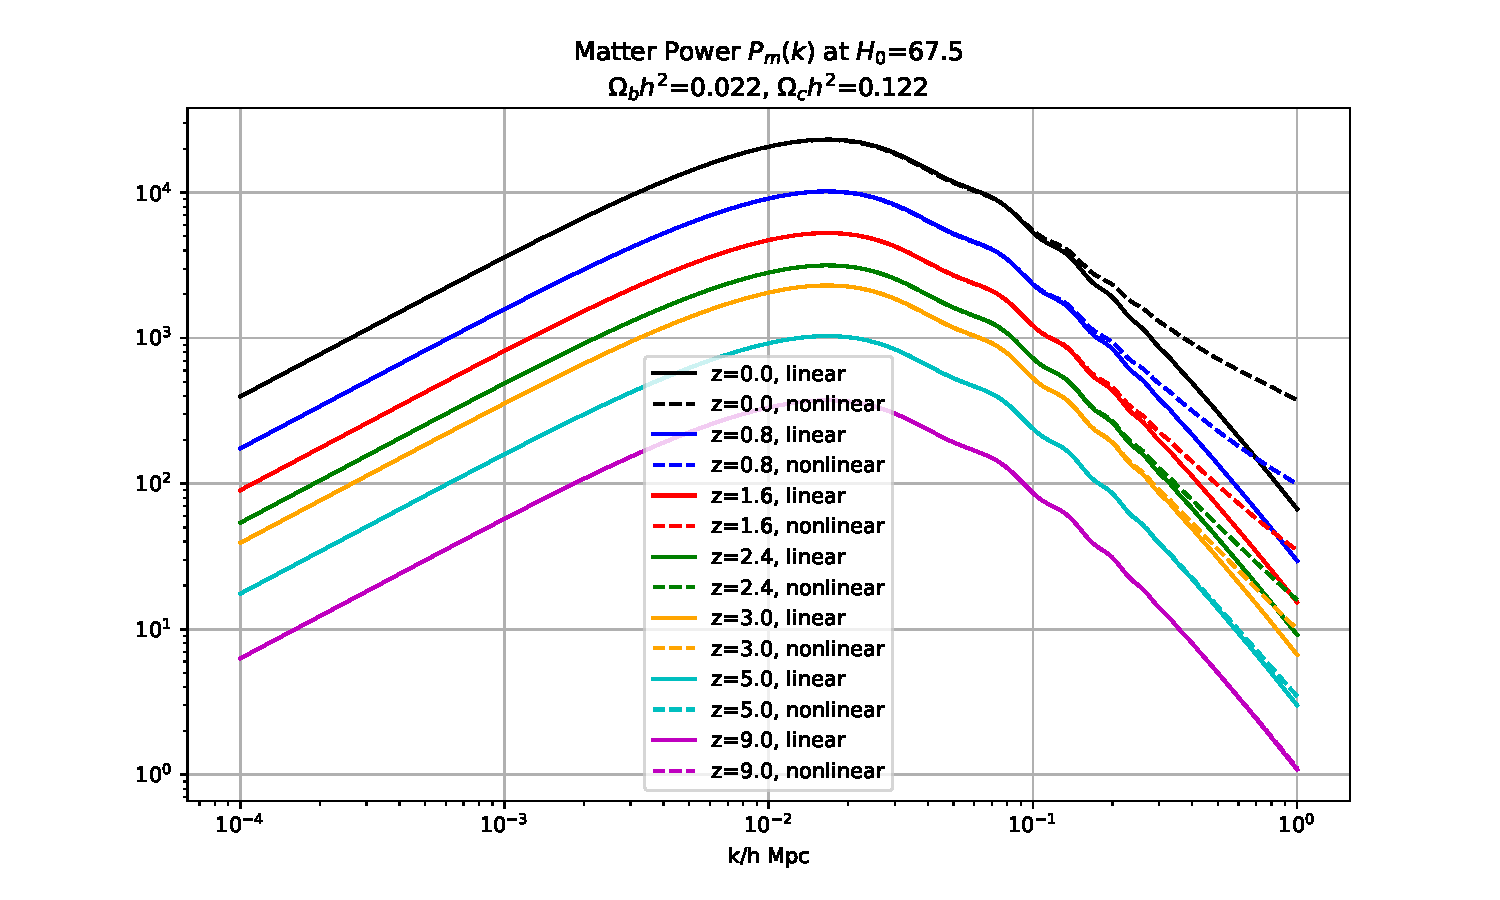
\includegraphics[width=\linewidth]{powerspectrum_var_z.pdf}
        \cprotect\caption{Varying Redshift $z$ (\verb|z|)}
    \end{subfigure}
    % Subfigure (b)
    \begin{subfigure}[b]{0.49\textwidth}
        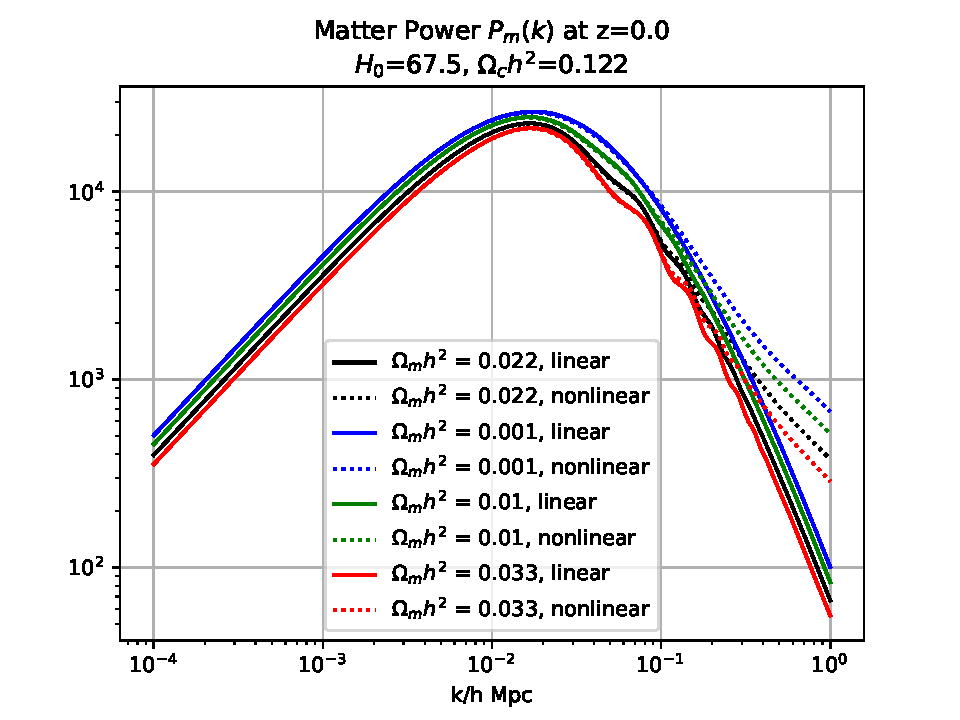
\includegraphics[width=\linewidth]{powerspectrum_var_baryonic_density.pdf}
        \cprotect\caption{Varying Baryonic Matter Density $\Omega_m h^2$ (\verb|ombh2|)}
    \end{subfigure}
    % Subfigure (c)
    \begin{subfigure}[b]{0.49\textwidth}
        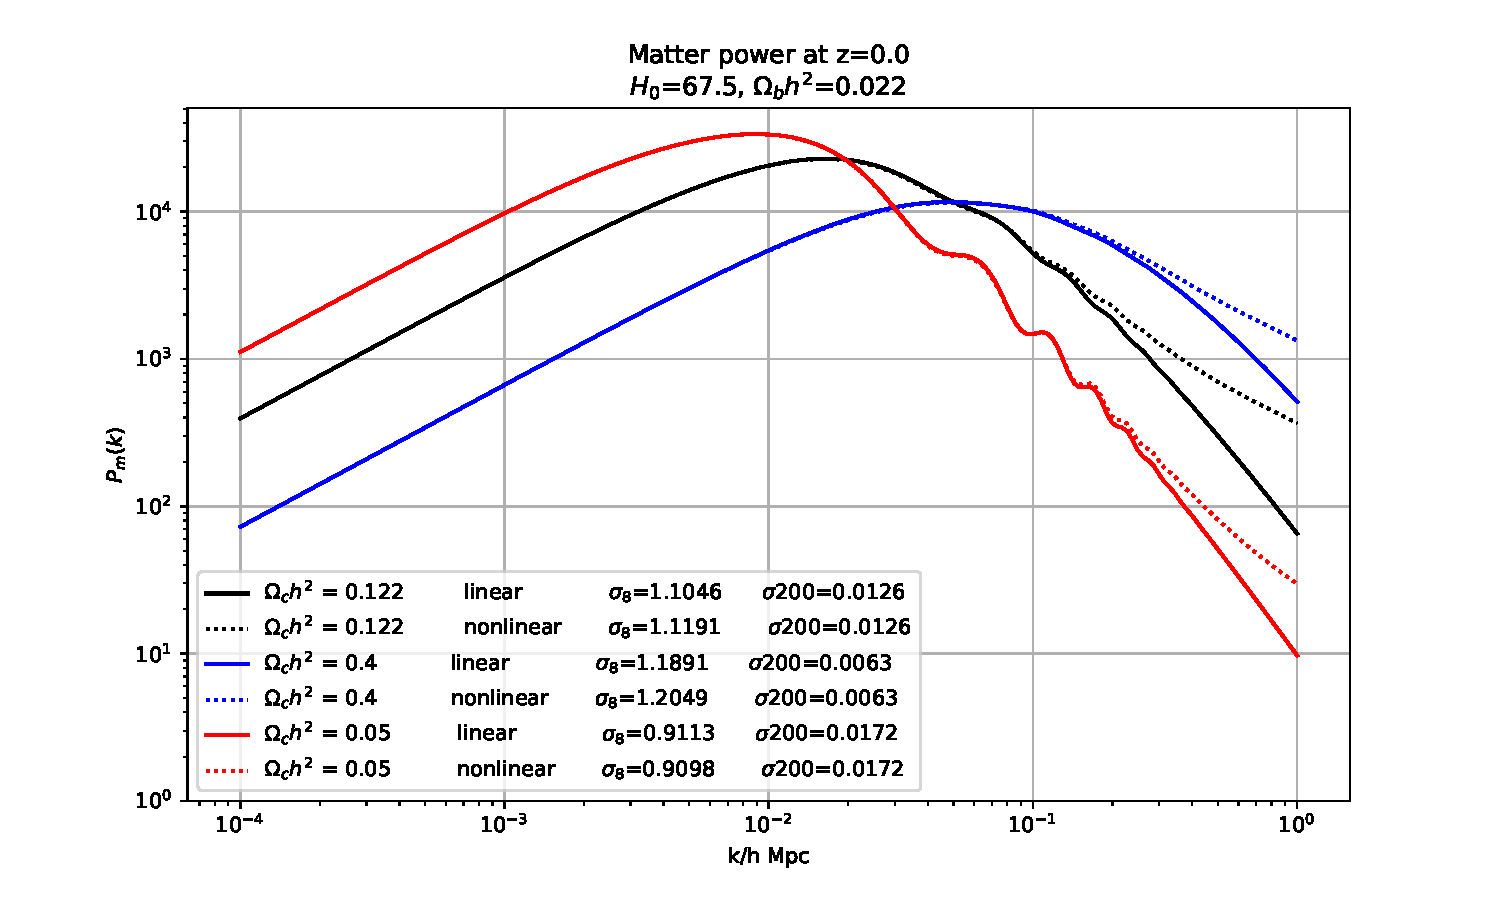
\includegraphics[width=\linewidth]{powerspectrum_var_cdm_with_sigma.pdf}
        \cprotect\caption{Varying CDM Density $\Omega_c h^2$ (\verb|omch2|)}
    \end{subfigure}
    % Subfigure (d)
    \begin{subfigure}[b]{0.49\textwidth}
        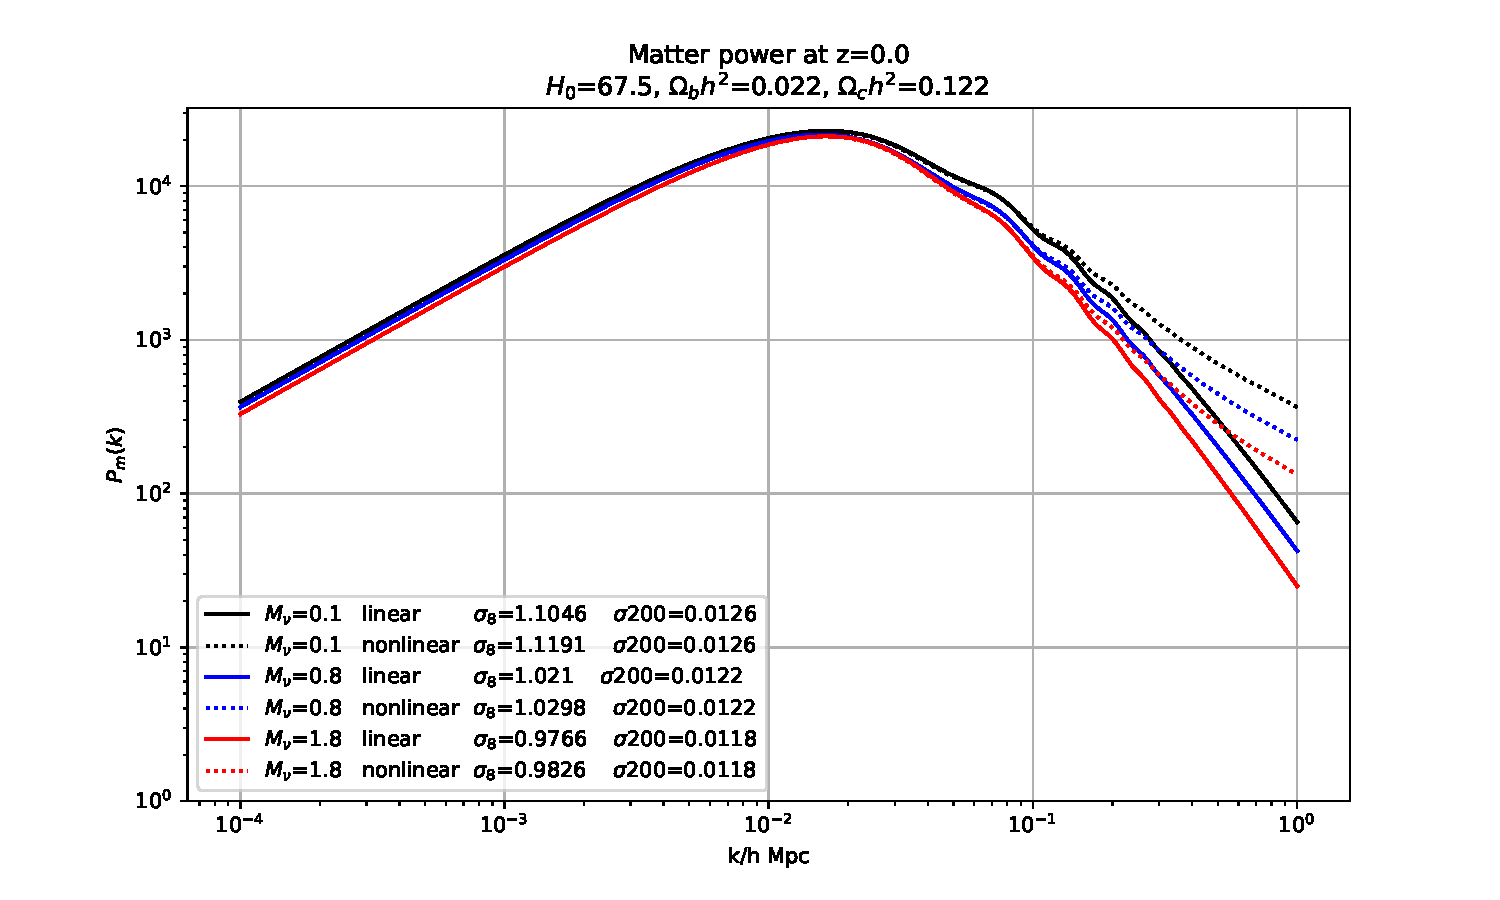
\includegraphics[width=\linewidth]{powerspectrum_var_mnu_with_sigma.pdf}
        \cprotect\caption{Varying Total Neutrino Mass$M_\nu$ (\verb|mnu|)}
    \end{subfigure}
    \caption{Matter power spectrum $P_m(k)$ while varying different parameters}
    \label{fig:powerspectrum_var_par}
\end{figure}

As shown in Figure \ref{fig:powerspectrum_var_par} (a), as redshift $z$ increases, the magnitude of the curve get smaller, but the amount that it gets smaller also becomes smaller with higher $z$. In Figure 2 (b), ~$0.01$ difference in \verb|ombh2| results in 10\% or less difference in the magnitude of the curves. However, in Figure 2 (c), while \verb|omch2| = 0.05 has a very strong nonlinear effect for large $k$ values, \verb|omch2| = 0.4 is very smooth and the peak of the curve shifts towards the right as \verb|omch2| increases. For Figure 2 (d), the story is somewhat similar to Figure 2 (a). In all of the cases, the nonlinear growth becomes dominant for $k$ beyond around $10^{-2}$. \\

Another method of displaying the power spectrum is to use the "dimensionless" power spectrum $\Delta^2(k)$:
% Dimensionless power spectrum (1)
\begin{equation}
    \Delta^2(k) \equiv k^3 P_m(k) / (2\pi^2)
\end{equation}
Figure \ref{fig:powerspectrum_dimensionless} shows the graph of $\Delta^2(k)$ vs. $k$ for standard cosmological parameters. There is a clear deviation between the linear and the nonlinear effect starting from the point where $\Delta^2 = 1$ at $k\approx0.2$. The values of $k$ where $\Delta^2(k) = 1$, plotted in Figure \ref{fig:powerspectrum_dimensionless} in yellow, are:
\begin{align*}
    k_{linear} = 0.2495 \\
    k_{nonlinear} = 0.2073.
\end{align*}

% Figure 3
\begin{figure}[h!]
    \centering
    \includegraphics[scale=0.5]{DimensionlessMatterPowerSpectra.pdf}
    \caption{Dimensionless Power Spectrum\\$\Delta^2 = 1$ at around $k \approx 0.2$}
    \label{fig:powerspectrum_dimensionless}
\end{figure}

The variance of a cosmic density field that is smoothed within spheres of radius R (in units of $h^{-1} Mpc$) is given by
% Variance sigma R (2)
\begin{equation}
    \sigma^2_R = \int^\infty_0 \left[ \frac{3j_1(kR)}{kR}\right]^2 \frac{\Delta^2(k)}{k} dk
    \label{eqn:sigmaR}
\end{equation}
where $W(k,R) \equiv \frac{3j_1(kR)}{kR}$ and $j_1$ is the first spherical Bessel function, $j_1(x) = \frac{sin(x)}{x^2} - \frac{cos(x)}{x}$.\\
Figure 4 shows the plot of $W(k,R)$ for $R = 8 h^{-1} Mpc$ and $R = 200 h^{-1} Mpc$.

% Figure 4
\begin{figure}[h!]
    \centering
    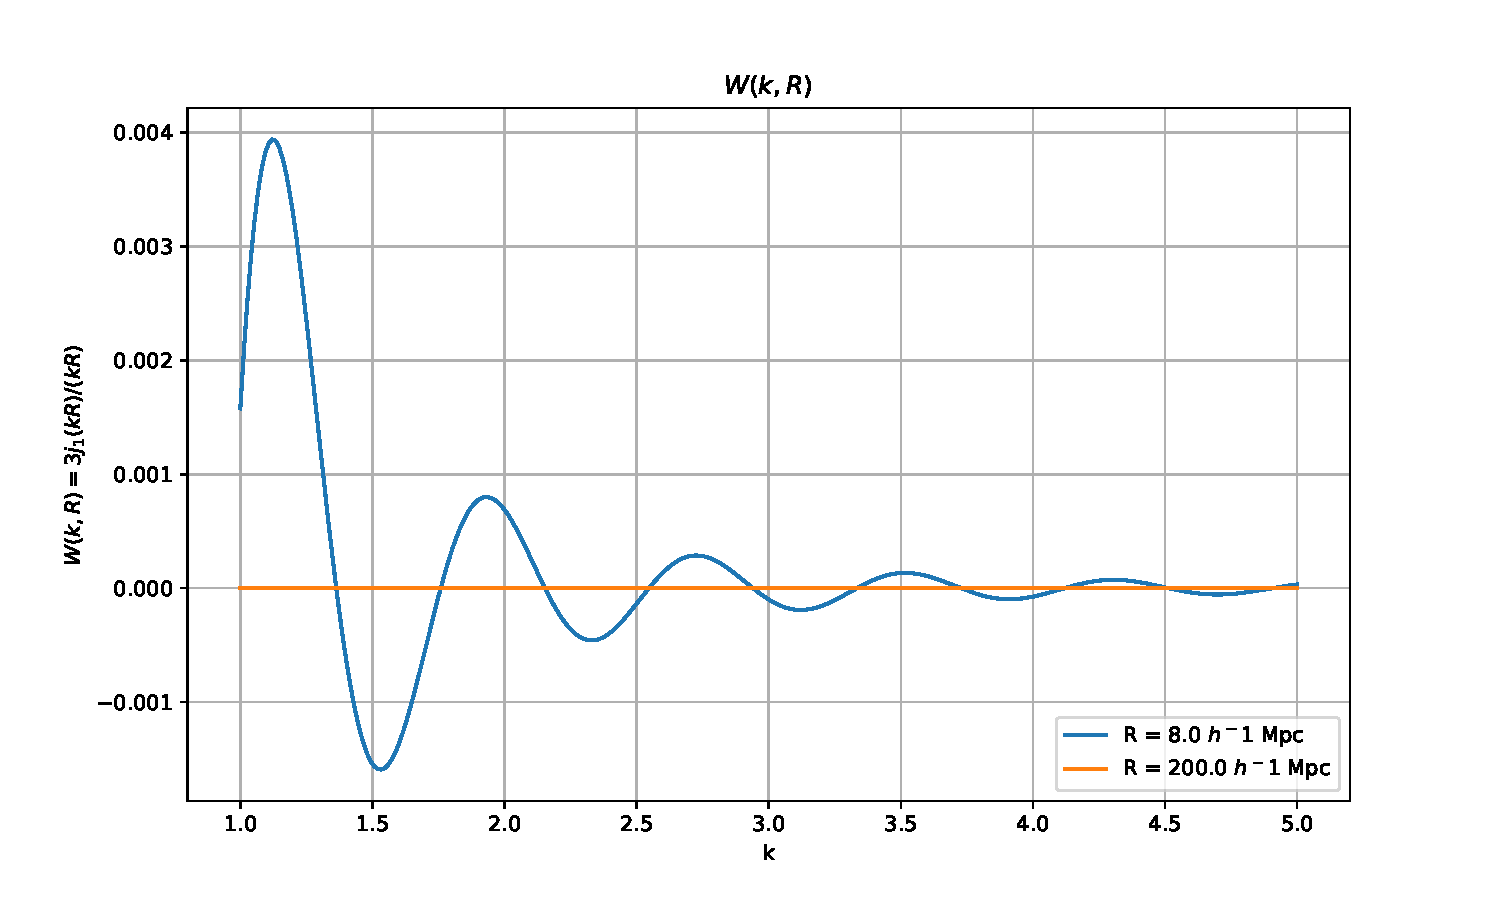
\includegraphics[scale=0.4]{W_kR.pdf}
    \caption{$W$ for $R = 8 h^{-1} Mpc$ and $R = 200 h^{-1} Mpc$}
    \label{fig:W_kR}
\end{figure}
\noindent
For $R = 200 h^{-1} Mpc$, $W$ is minuscule everywhere, and hence the integrand in Equation \ref{eqn:sigmaR} will be very small, further resulting in a very tiny variance. This relates to the fact that for $R$ very large, most of the small scale structures have been smoothed, making the universe nearly homogeneous (hence small variance in the matter density). \\\\

Plotting the variance $\sigma_R$ as a function of the smoothing sphere radius $R$ at redshift $z = 0$, we obtain the following:
% Figure 5
\begin{figure}[h!]
    \centering
    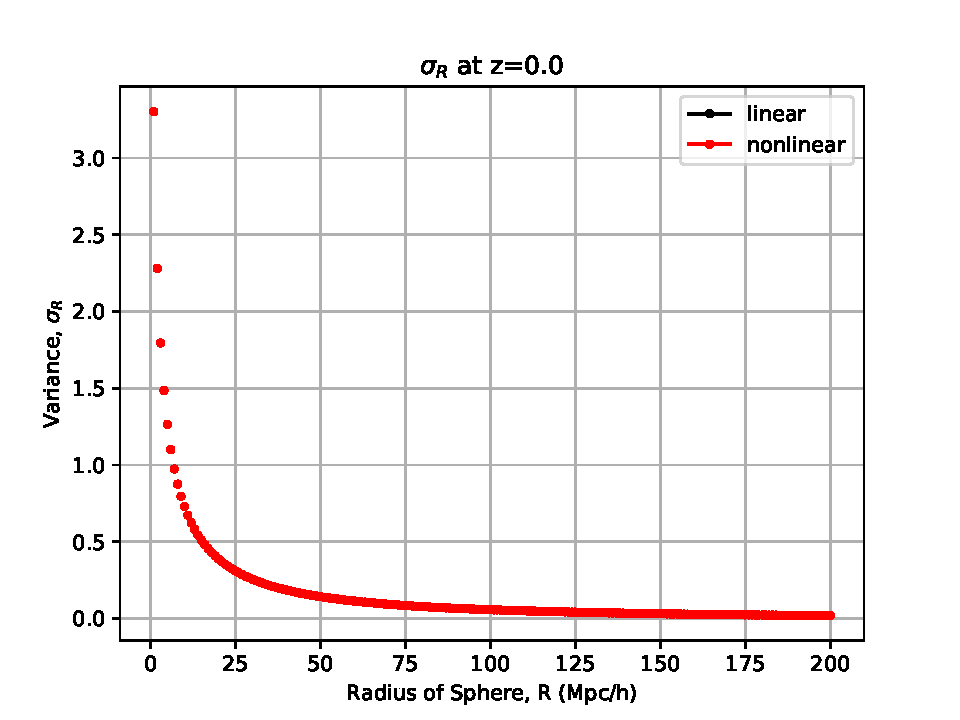
\includegraphics[scale=0.4]{sigma_R.pdf}
    \caption{$\sigma_R$ as a function of smoothing sphere radius $R$ at $z = 0$\\for linear and nonlinear growth}
    \label{fig:sigma_R}
\end{figure}

Computing the variance at $R = 8 h^{-1} Mpc$ and $R = 200 h^{-1} Mpc$ for the same curves obtained in Figure 2:

% Figure 6
\begin{figure}[h!]
    \centering
    % Subfigure (a)
    \begin{subfigure}[b]{0.49\textwidth}
        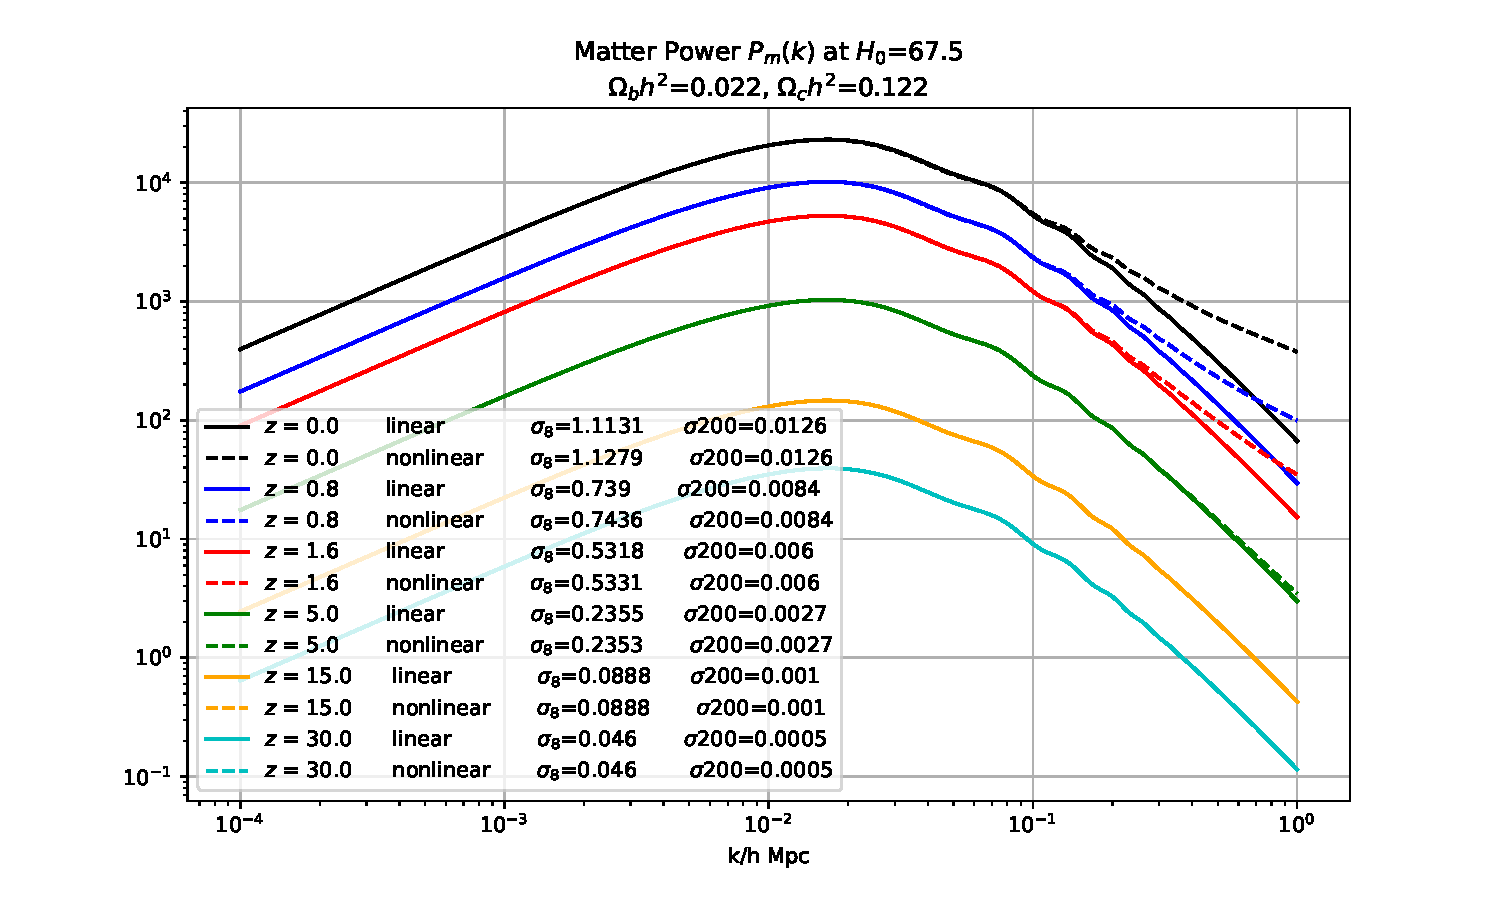
\includegraphics[width=\linewidth]{powerspectrum_var_z_with_sigma.pdf}
        \cprotect\caption{Varying Redshift $z$ (\verb|z|)}
    \end{subfigure}
    % Subfigure (b)
    \begin{subfigure}[b]{0.49\textwidth}
        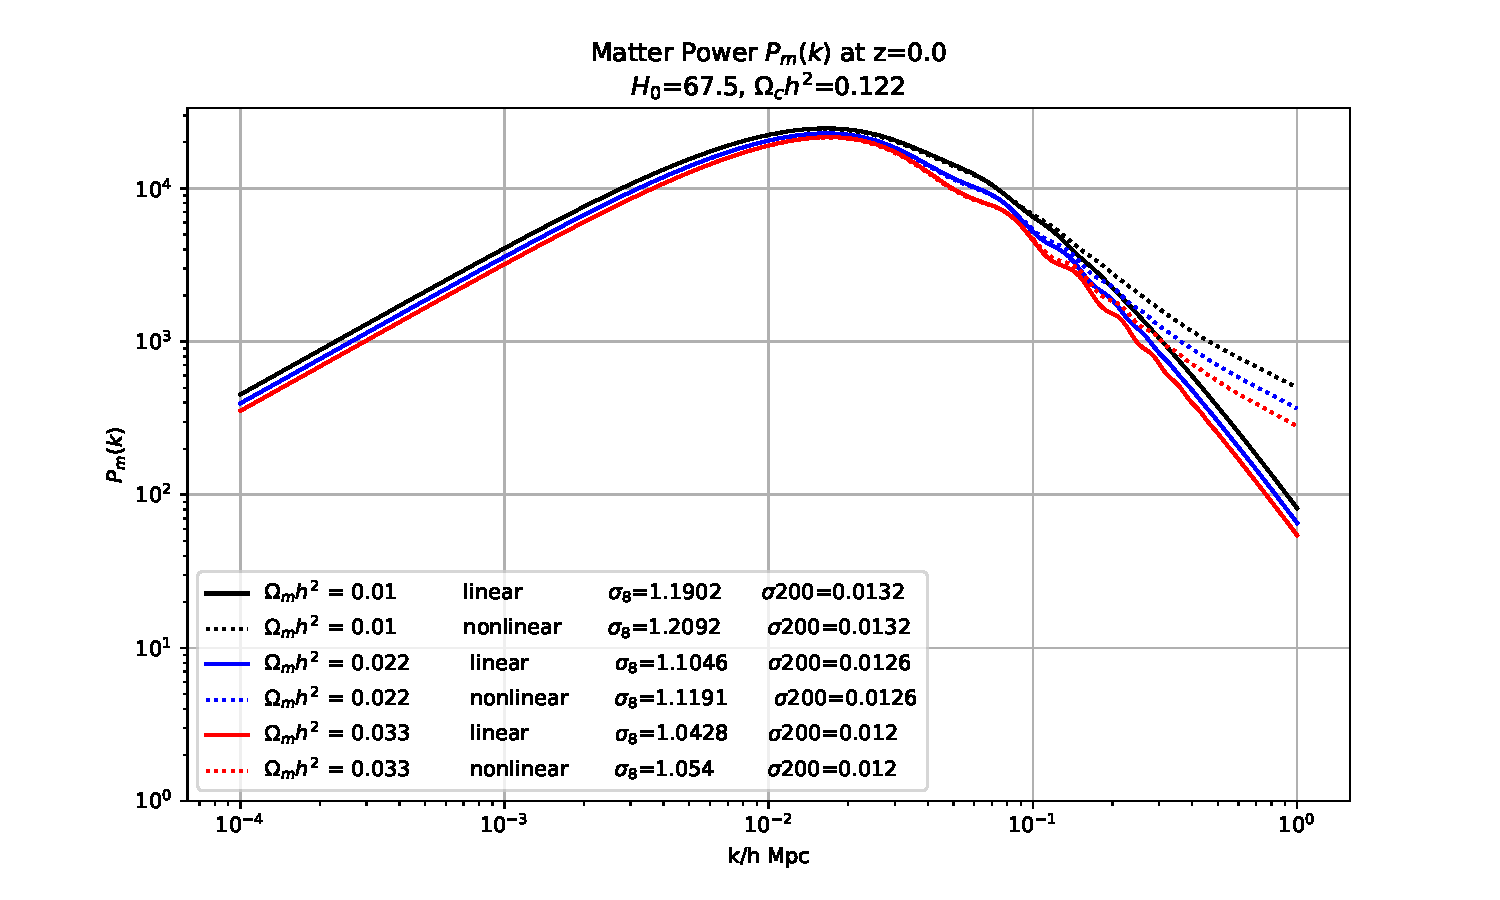
\includegraphics[width=\linewidth]{powerspectrum_var_baryonic_density_with_sigma.pdf}
        \cprotect\caption{Varying Baryonic Matter Density $\Omega_m h^2$ (\verb|ombh2|)}
    \end{subfigure}
    % Subfigure (c)
    \begin{subfigure}[b]{0.49\textwidth}
        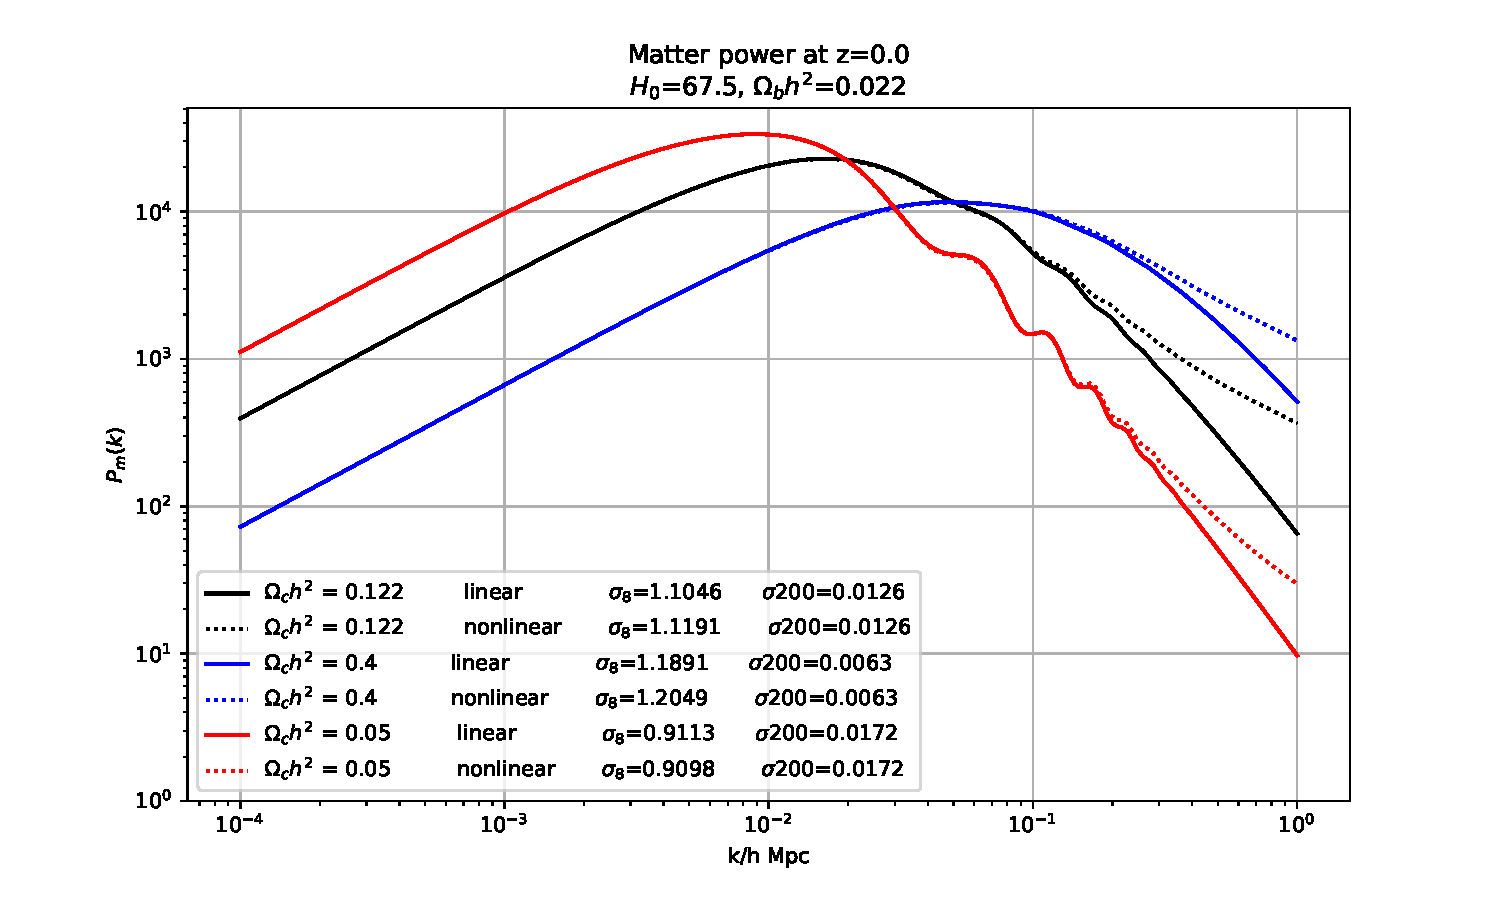
\includegraphics[width=\linewidth]{powerspectrum_var_cdm_with_sigma.pdf}
        \cprotect\caption{Varying CDM Density $\Omega_c h^2$ (\verb|omch2|)}
    \end{subfigure}
    % Subfigure (d)
    \begin{subfigure}[b]{0.49\textwidth}
        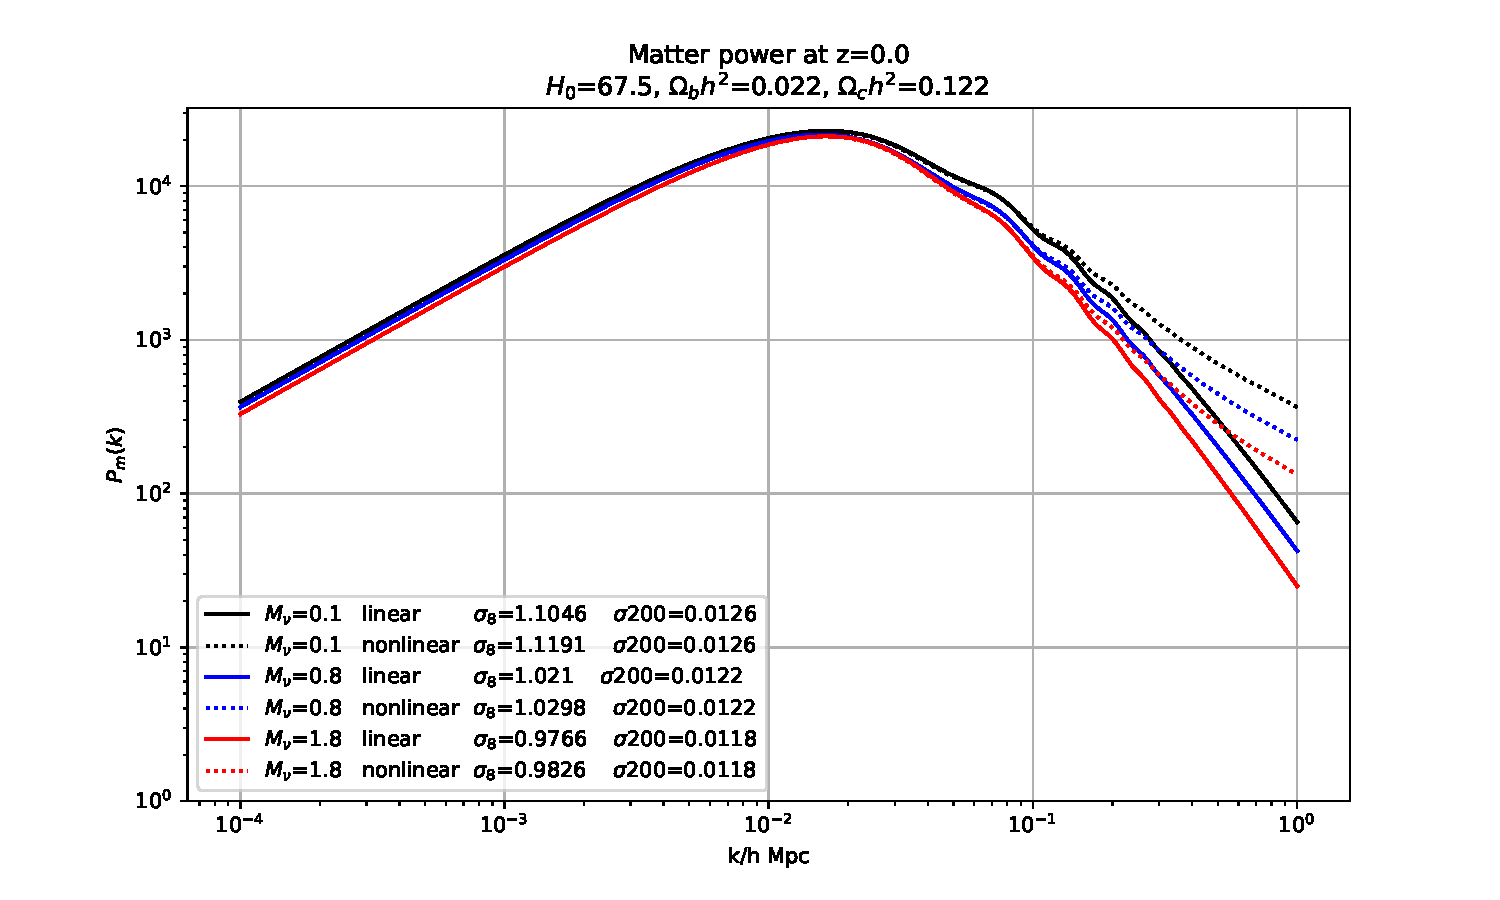
\includegraphics[width=\linewidth]{powerspectrum_var_mnu_with_sigma.pdf}
        \cprotect\caption{Varying Total Neutrino Mass$M_\nu$ (\verb|mnu|)}
    \end{subfigure}
    \caption{Matter power spectrum $P_m(k)$ while varying different parameters}
    \label{fig:powerspectrum_var_par}
\end{figure}



\newpage
% Question 2
\section{Generating and Analyzing Simulations of Clustering}
In this section, the \verb|nbodykit| is used to simulate many particles and calculate their power spectrum. The \verb|nbodykit| uses the data structure \verb|catalog| to store information about each of the cosmological objects, and \verb|mesh| to store these information in a discretized array space. 

% Question 2 Part 3
\paragraph{Gaussian Random Field:} Here, we simulated the universe where the mass density of the particles follow a Gaussian random field (GRF). 10 realizations of GRF are made with a \verb|mesh| in a box with side lengths $L = 1000 h^{-1} Mpc$ on a $256^3$ mesh. For each of the realizations, two – a linear and a nonlinear growth – power spectra are computed at redshifts $z = 0$ and $z = 5$, as well as the mean and standard deviation between the 10 instances as a function of wavenumber $k$.

% Figure 7
\begin{figure}[h!]
    \centering
    % Subfigure (a)
    \begin{subfigure}[b]{0.49\textwidth}
        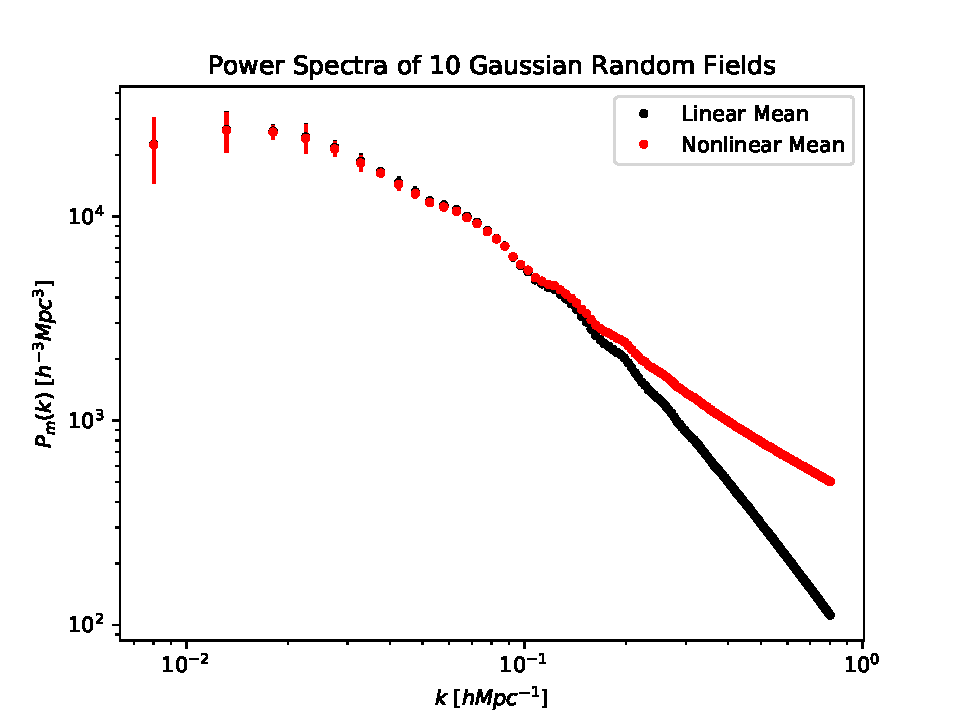
\includegraphics[width=\linewidth]{mean_power.pdf}
        \cprotect\caption{$z = 0$\\(with standard deviation $\sigma$)}
    \end{subfigure}
    % Subfigure (b)
    \begin{subfigure}[b]{0.49\textwidth}
        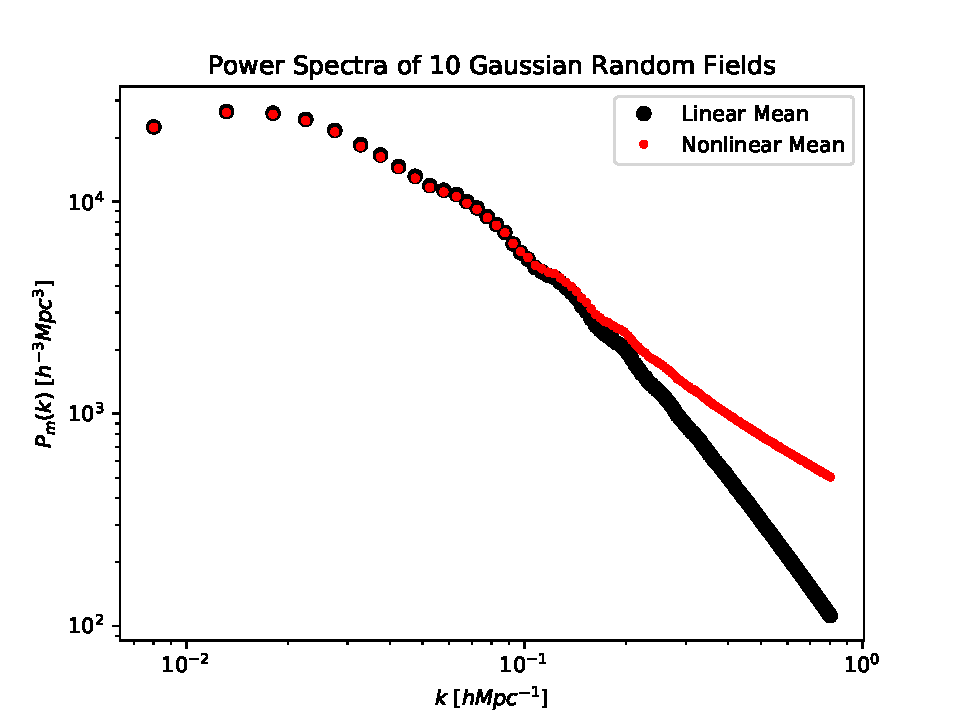
\includegraphics[width=\linewidth]{mean_power5.pdf}
        \cprotect\caption{$z = 5$\\(without standard deviation $\sigma$)}
    \end{subfigure}
    \cprotect\caption{Mean Power Spectra for GRF for Linear and\\ Nonlinear Growth at Redshifts $z = 0$ and $z = 5$}
    \label{fig:MeanGRF}
\end{figure}

\noindent{Figure \ref{fig:MeanGRF} shows the mean linear and nonlinear power spectra using the GRF distribution of mass, at $z = 0$ in Fig. 7 (a), and at $z = 5$ in Fig. 7 (b). The linear power spectrum was obtained using the \verb|LinearPower| method, while the nonlinear power spectrum was obtained using the \verb|HalofitPower| method. Firstly, for low $k$, the linear and nonlinear power spectra do not have a clear difference as it does for high $k$, where the nonlinear curve starts to pick up and stops decreasing as much as the linear curve, which keeps decreasing logarithmically. Between the two redshifts, there is no significant difference in their corresponding power spectra for linear and nonlinear curves. However, in either case, there is a large deviation between the 10 realizations for very small $k$, but eventually becomes identical above $k \approx 10^{-1}$.} \\

% Question 2 part 4
\paragraph{Lognormal Density Distribution Field:}Here, we study the simulation of particles whose density follow a lognormal statistics, as in the case of gravitational evolution of particles. Similar to GRF simulations, we generate 10 lognormal distribution of particles, but this time as \verb|catalog|s instead of \verb|mesh|es. Again, the box has side lengths $L = 1000 h^{-1} Mpc$ on a $256^3$ mesh, with $\bar{n} = 3\times 10^{-3} h^3 Mpc^{-3}$, which is the number density of the particles in the box.\\

In order to numerically compute the power spectrum, the \verb|catalog| object must be discretized into a \verb|mesh| object. During this process, the number density of the particles that fall within each grid of the mesh gets averaged, or 'smoothed' throughout that voxel. This effectively is a convolution process with a window function, hence in order to get back the original power spectrum corresponding to the \verb|catalog| object, the resulting power spectrum must be deconvoluted. The \verb|FFTPower| function can take a number of these 'window functions'. We try the \verb|CIC| and \verb|TSC| options for the window parameter (\verb|NGP| is nowhere to be found on the \verb|nbodykit| website).\\

Figure \ref{fig:mean_CIC_TSC} shows the two plots in which for each, the linear power spectrum with and without the window function deconvolution option are shown. The black points show the linear power spectrum when the window function deconvolution was applied to achieve back the power spectrum, and the red points show the same linear power spectrum without applying such deconvolution. Figure \ref{fig:mean_CIC_TSC} (a) shows the plot using the \verb|CIC| window function, and (b) shows the plot using the \verb|TSC| window function option. The red curve in the two plots should be identical. It can be seen that there are no significant differences between the two window function options, including the standard deviation for each $k$.

% Figure 8
\begin{figure}[h!]
    \centering
    % Subfigure (a)
    \begin{subfigure}[b]{0.49\textwidth}
        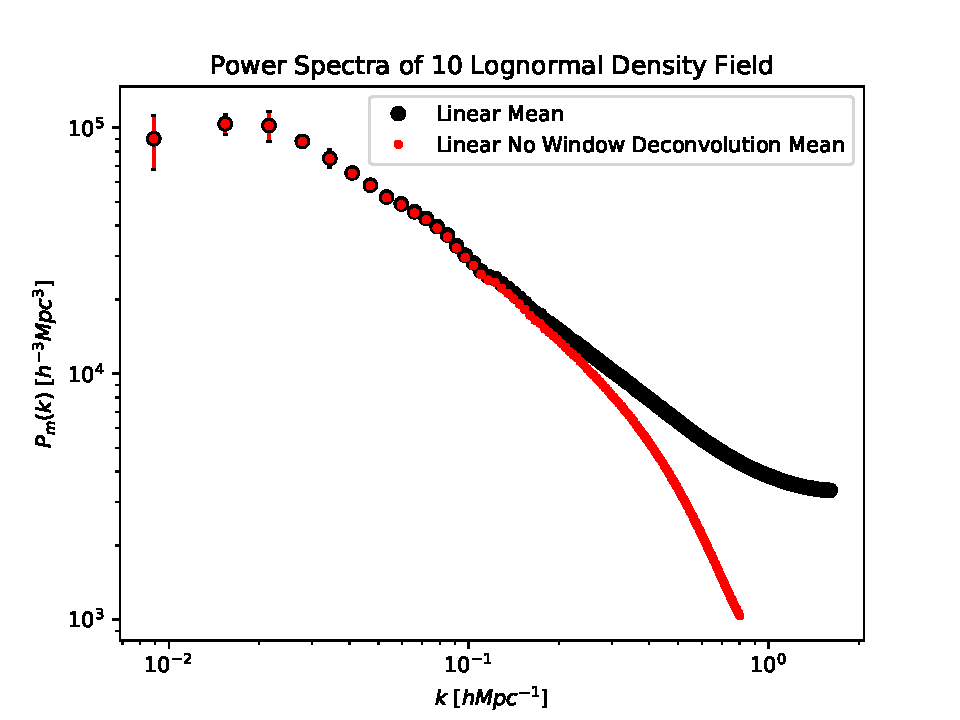
\includegraphics[width=\linewidth]{mean_power_lognormal_with_nowind_cic.pdf}
        \cprotect\caption{CIC}
    \end{subfigure}
    % Subfigure (b)
    \begin{subfigure}[b]{0.49\textwidth}
        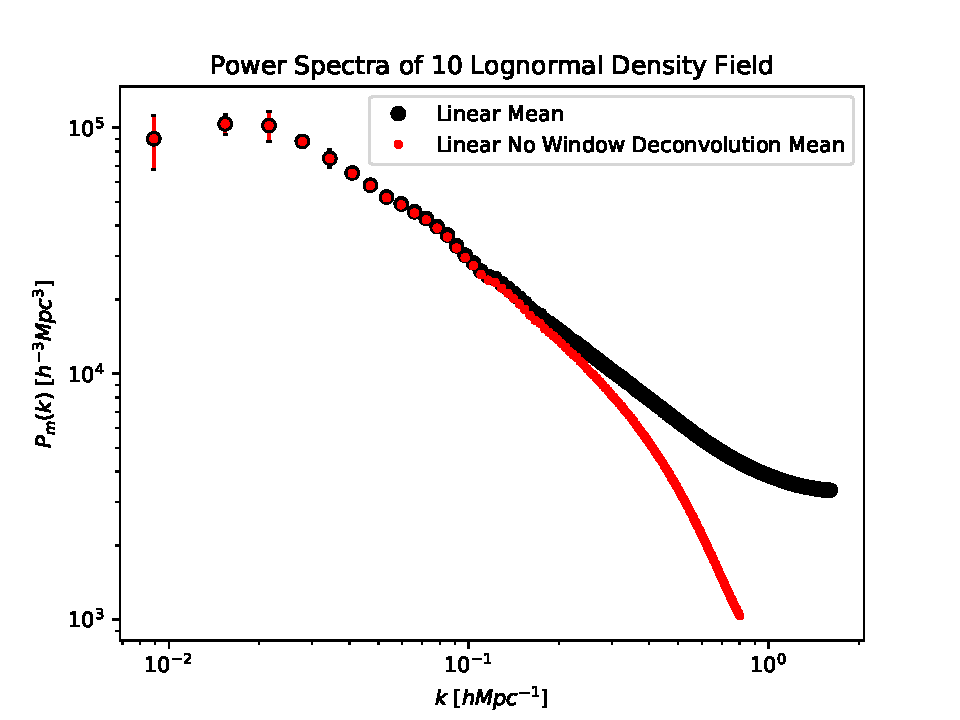
\includegraphics[width=\linewidth]{mean_power_lognormal_with_nowind_tsc.pdf}
        \cprotect\caption{TSC}
    \end{subfigure}
    \cprotect\caption{Mean Matter Power Spectrum for Lognormal Field with \\(and without) \verb|CIC| and \verb|TSC| Window Function Deconvolution}
    \label{fig:mean_CIC_TSC}
\end{figure}

We then vary the number density of the particles $\bar{n}$ to $1\times10^{-3}$, $5\times10^{-4}$, and $1\times10^{-4} h^3 Mpc^{-3}$. Figure \ref{fig:mean_nbar} shows the plots for different $\bar{n}$'s. It seems that for all curves except $\bar{n} = 1\times10^{-4} h^3 Mpc^{-3}$ in Fig. 9 (d), the power spectra values for low $k$'s are more or less the same - the one in Fig. (d) is about 10\% higher than the rest. However, in the high $k$ regime, the four values of $\bar{n}$ results in drastically different behaviours for the deconvoluted linear mean power spectra, with $\bar{n} = 3\times10^{-3}$ and $5\times10^{-4} h^3 Mpc^{-3}$ tapering off at a similar magnitude of the power spectrum value ($P_m(k)\approx2\times 10^{3} h^{-3} Mpc^{3}$) while $\bar{n} = 1\times10^{-3}h^3 Mpc^{-3}$ tapers off at a lower $P_m(k)\approx1\times 10^{3} h^{-3} Mpc^{3}$ and $\bar{n} = 1\times10^{-4}h^3 Mpc^{-3}$ tapering off an order of magnitude higher at $P_m(k)\approx1\times 10^{4} h^{-3} Mpc^{3}$. 

\newpage
% Figure 9
\begin{figure}[t!]
    \centering
    % Subfigure (a)
    \begin{subfigure}[b]{0.49\textwidth}
        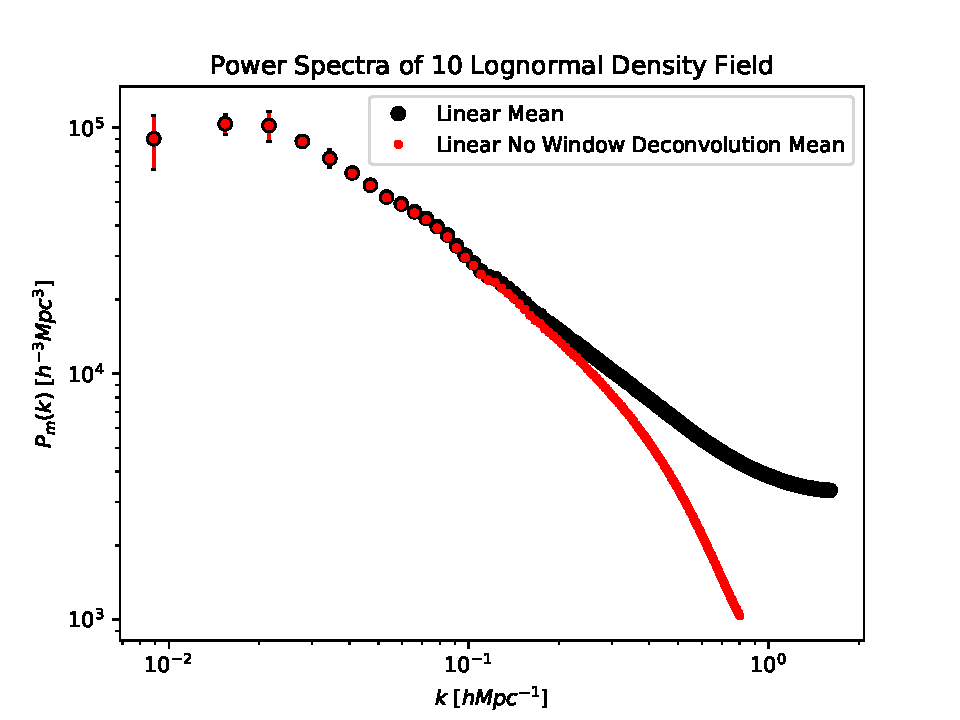
\includegraphics[width=\linewidth]{mean_power_lognormal_with_nowind_cic.pdf}
        \cprotect\caption{$\bar{n} = 3\times10^{-3}h^3Mpc^{-3}$\\}
    \end{subfigure}
    % Subfigure (b)
    \begin{subfigure}[b]{0.49\textwidth}
        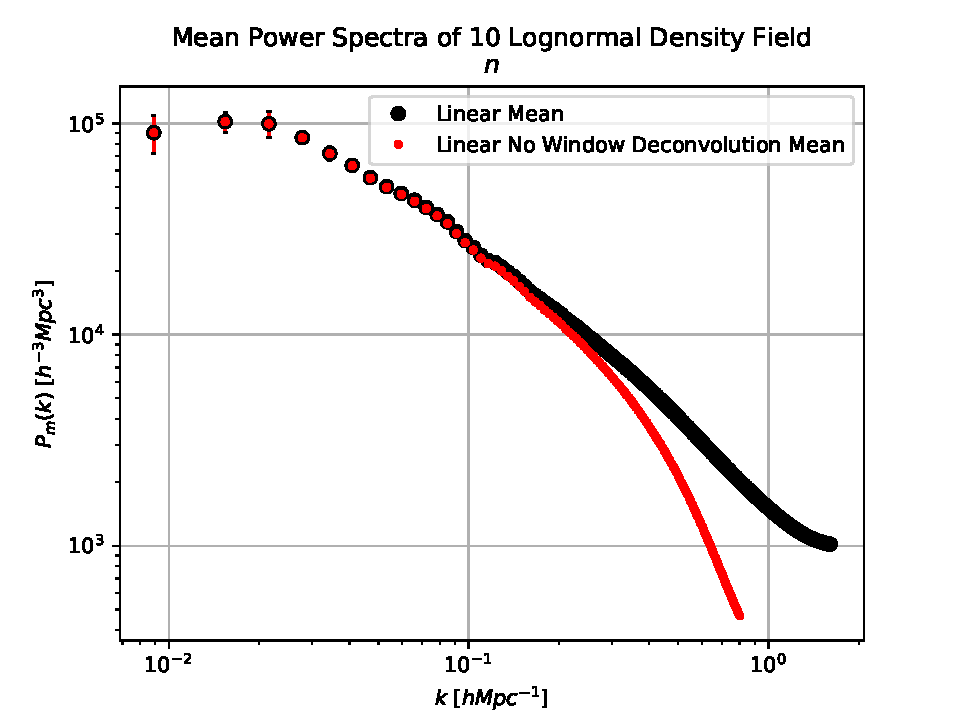
\includegraphics[width=\linewidth]{mean_power_lognormal_with_nowind_CIC_nbar1e-3.pdf}
        \cprotect\caption{$\bar{n} = 1\times10^{-3}h^3Mpc^{-3}$\\}
    \end{subfigure}
    % Subfigure (c)
    \begin{subfigure}[b]{0.49\textwidth}
        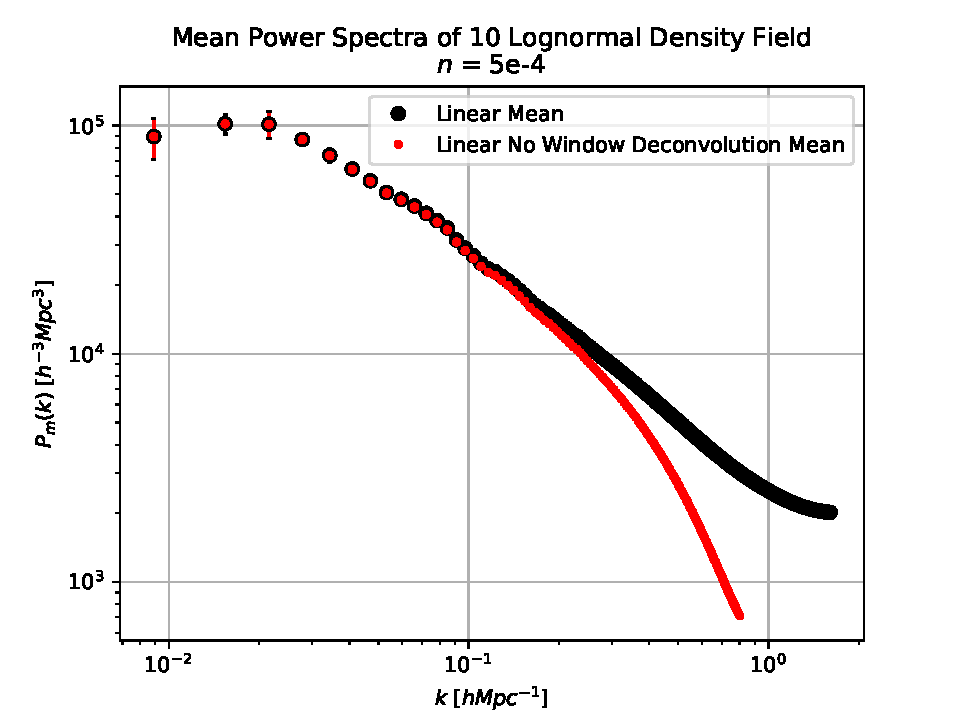
\includegraphics[width=\linewidth]{mean_power_lognormal_with_nowind_CIC_nbar5e-4.pdf}
        \cprotect\caption{$\bar{n} = 5\times10^{-4}h^3Mpc^{-3}$}
    \end{subfigure}
    % Subfigure (d)
    \begin{subfigure}[b]{0.49\textwidth}
        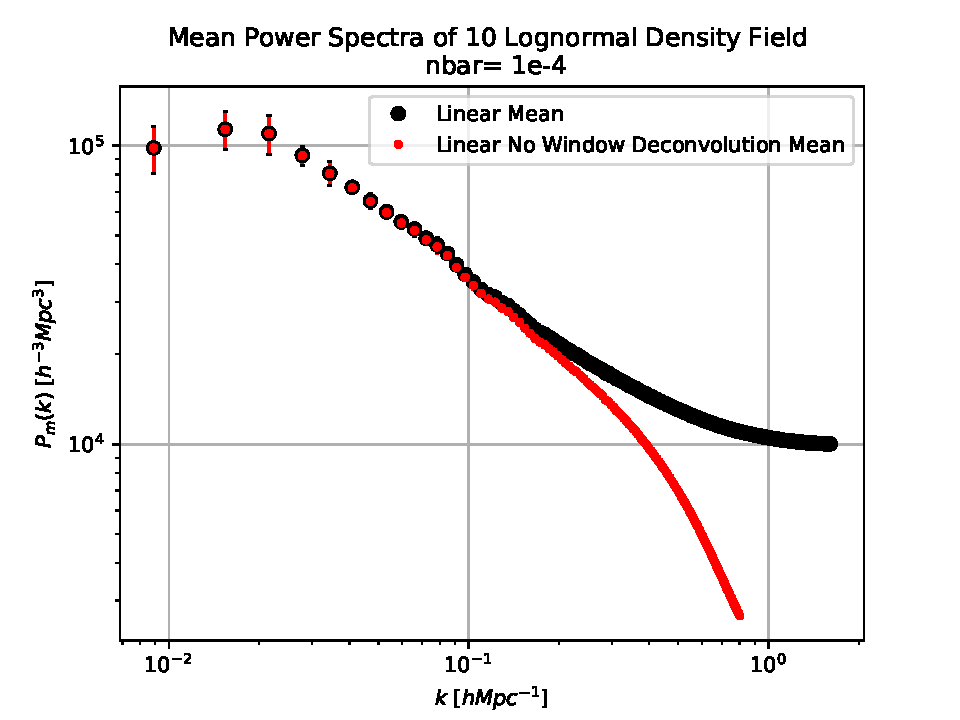
\includegraphics[width=\linewidth]{mean_power_lognormal_with_nowind_CIC_nbar1e-4.pdf}
        \cprotect\caption{$\bar{n} = 1\times10^{-4}h^3Mpc^{-3}$}
    \end{subfigure}
    \cprotect\caption{Mean Power Spectrum for Lognormal Field with \verb|CIC| Window Function Deconvolution\\for $\bar{n} = 3\times10^{-3}h^3Mpc^{-3}$, $1\times10^{-3}$, $5\times10^{-4}$, and $1\times10^{-4} h^3Mpc^{-3}$}
    \label{fig:mean_nbar}
\end{figure}

From this study we have learned that at low values of $k$, the nonlinear growth does not have much affect on the power spectra, but at high $k$, this effect becomes dominant and must be accounted for. It is also blatantly clear that the deconvolution process is a must, since without it, the power spectrum exhibits a behaviour similar to not accounting for the nonlinear growth. The window function for deconvolution, \verb|CIC| and \verb|TSC|, however, did not seem to matter too much, as well as small differences in redshifts $z = 0$ and $z = 5$.

\end{document}

